\documentclass[fleqn,10pt,lineno]{wlpeerj}

\title{Functional boxplots for epidemic and other data: extensions of Juul \emph{et al.} (2021)}
%  Additional details on centrality measure of epidemic functional data

\author[1]{Ali Gharouni}
\author[1,2,3]{Benjamin M. Bolker}
\affil[1]{Department of Mathematics \& Statistics, McMaster University, Hamilton, Canada}
\affil[2]{Department of Biology, McMaster University, Hamilton, Canada}
\affil[3]{Michael G. DeGroote Institute for Infectious Disease Research, McMaster University, Hamilton, Canada}
\corrauthor[1]{First Author}{agharoun@uottawa.ca \footnote{
The auther is currently at the Department of Mathematics and Statistics, University of Ottawa.}}

% \keywords{Statistical depth, Functional depth, Functional boxplot, Centroid}

\begin{abstract}
  The \emph{central set} of an ensemble of epidemic curves (or more generally of any functional data set) helps characterize the variation of the ensemble, which in turn gives insights into disease dynamics and management. Classical fixed-time descriptions of uncertainty such as pointwise confidence envelopes may be unreliable. Juul \emph{et al} 2021 described robust curve-based descriptive methods based on \emph{functional band depth} (FBD) to visualize the uncertainty associated with ensembles of epidemic curves from stochastic epidemic models. Extending and describing this approach further, we studied several different approaches to construct and visualize uncertainty regions. First, we compared curves using  Juul \emph{et al}'s FBD approach with a more widely used, computationally efficient implementation of FBD. Second, we developed a new centrality measure that uses a set of features of interest (such as the initial growth rate, peak time and peak height of the epidemic), combined into a Mahalanobis distance from the ensemble's centroid. Both methods provide useful results.
\end{abstract}

\begin{document}

\flushbottom
\maketitle
\thispagestyle{empty}

\section*{Introduction}

Summarizing the uncertainty for ensembles of curves generated by stochastic epidemic models can provide useful insight into the dynamics and management of epidemics. For these and other sets of \emph{functional data} --- data where each observation represents a continuous curve, computing the typical set of observations forms a basis for graphical and quantitative summaries. Computations of central sets rely in turn on robust and computationally efficient estimation methods.

\cite{juul2021fixed} pointed out shortcomings of the standard methods that researchers use to draw confidence intervals for ensembles of curves, with specific examples drawn from the output of stochastic epidemic models (also, see Appendix 2 in \cite{kiss2017mathematics}'s book). In particular, they showed that fixed-time approaches (e.g., computing pointwise quantiles) can fail to capture the uncertainty in key features of an epidemic such as the timing and magnitude of epidemic peaks.  As an alternative to fixed-time approaches, the authors illustrated methods to compute the \emph{central set} of an ensemble of curves, a high-dimensional analogue of interquartile range or confidence interval. A large body of literature addresses this topic under the rubrics of \emph{functional depth} and \emph{functional boxplots} for high dimensional data \citep{fraiman2001trimmed, lopez2007depth, lopez2009concept, sun2011functional,sun2012exact}. While \juul do cite this literature \citep{sun2011functional}, exploring it in more depth led us to several useful practical and theoretical points that could be useful for researchers interested in visualizing confidence regions for ensembles of curves.

In univariate data, the central set (region) can be easily represented by summaries based on univariate quantiles. Classical boxplots provide a visual summary of the data that represents the uncertainty (the range of the central set) by the interquartile range. In multivariate data, computing the central set relies on the concept of \emph{statistical depth} \citep{mahalanobis1936generalized, tukey1975mathematics, oja1983descriptive, liu1990notion, singh1991notion, vardi2000multivariate, zuo2003projection}. When generalized to functional data, the statistical depth is usually referred to as \emph{functional depth} \citep{fraiman2001trimmed}.
Roughly speaking, a functional depth is a bounded non-negative function which measures the average closeness of a function (in practice, one observation in a data set or curve in an ensemble) to all other functions, over a function-valued distribution (\citep{zuo2000general} gives formal definitions). 
One can then order the elements of an ensemble according to decreasing depth values, ranking the observations from the center (the deepest or most central point) outward, and define a central set that includes all the points up to a given depth or rank. The functional boxplot displays an ensemble in a way that highlights this central set. \citep{sun2011functional,sun2012exact}.
% BMB: why do we need this???
%In a recent work, \cite{wynne2021statistical} used a machine learning approache -- specifically, kernel mean embedding -- to study the functional depth.
 \cite{lopez2007depth} developed functional band depth (FBD), a sample-based method for determining a curve's centrality. FBD measures the fraction of times that a given curve is completely included within the envelope of a set of other curves randomly sampled from the ensemble. The sample size is determined by a \emph{tuning parameter} $J$, and one can take any number of samples up to the set of all possible combinations of size $J$. \juul used a version of FBD to create functional boxplots for an ensemble of epidemic curves simulated from a stochastic epidemic model. They chose $J=50$ (they use the notation \ncurve), and used $\nsample=100$ such samples to compute the FBD for each curve. They provided open-source Python code that implements this method, as well as some weighted variants of FBD. For the simple (unweighted) case, however, there are already mature open source implementations available in R \citep{fda_pkg,roahd}, Matlab (\url{https://www.psych.mcgill.ca/misc/fda/downloads/FDAfuns/}), and Python \citep{seabold2010statsmodels}. In general these packages use the same functional band depth measure as \juul, but substituting $J=2$, which is robust \citep{lopez2009concept} and allows the use of a computationally efficient algorithm for large data sets \citep{sun2012exact}. It is unclear why \juul chose larger values of $J$ (10 and 50), although the dimensions of their examples are small enough that the computational burden is not important.

\juul also suggest ranking according to a single, one-dimensional feature of interest such as the maximum values of newly hospitalized cases in a single day (their Fig.~2e). This approach can be extended to incorporate multiple features of interest. FBD can be based on this reduced set of features; here we use the \emph{Mahalanobis distance} \citep{mahalanobis1936generalized}, which measures distance from a centroid accounting both for variation in the scales or typical magnitudes of different features and for correlation among features. Our example uses a feature set including the peak value of incidence (new infections), the time at which the peak occurs, and the initial growth rate, duration, and final size of the epidemic. While these are typical epidemiological features of interest, researchers can and should choose the features that are most closely connected to their particular research questions \citep{probert2016decision}.

We compare the central set of the epidemic ensemble (provided in \juul's work) by defining various statistical depths and ranking the curves using (i) FBD with different choices of the tuning parameter $J$ to compare classical ($J=2$) with \juul's 2021 approach ($J=50$), and (ii) a functional depth measure based on Mahalanobis distances among features of interest.
Although we used an epidemic ensemble, our methods are broadly applicable to any functional data set.

\section*{Methods}

We present the comparison of 90\% central regions computed with different functional band depth methods. We apply our methods on \juul dataset (\url{https://github.com/jonassjuul/curvestat/tree/master/curvestat/tests/test_data}) and compare our results with theirs.

First, we implemented \juul's FBD method in R \citep{R}. In particular, the algorithm: (i) randomly samples a subset of curves from the ensemble ($J=50$), (ii) computes the envelopes (pointwise minima and maxima of the sample), (iii) scores all curves in the ensemble based on whether they lie entirely within the envelope (score=1) or not (score=0), and (vi) repeats (i)-(iii) to derive a rank, or depth, for each curve based on the average score. The central set consists of the curves above a specified depth.

Second, we used the function {\tt fda()} in the R package \pkg{roahd} \citep{roahd} to compute central sets, with the choice of modified band depth (MBD) to break ties which is based on the fast algorithm proposed by \cite{sun2012exact}.

Third, we computed central sets by defining a feature vector for each curve in the ensemble and computing the average pairwise Mahalanobis distances to every other point in the set, using the {\tt mahalanobis()} function in R and using the covariance matrix from the entire  set of features as the scaling factor. \textbf{why do we compute pairwise Mahalanobis distances rather than computing distances from the centroid, which is much more efficient and which we have established is equivalent to calculating the rank based on average pairwise distances???} The rank of each curve is the rank of its average distance to the rest of the set.

The ensemble of curves, which we took from \cite{juul2021fixed}'s supplementary data, represents the number of newly hospitalized people over time, which is a version of the epidemic incidence (typically measured by the number of new infections or number of newly detected cases).
In keeping with the epidemic-modeling focus, we chose the curve features as (i) the peak
hospitalization rate; (ii) the time at which the peak occurs; (iii) the initial growth rate; (iv) the epidemic duration; and (v) the total size of the epidemic (as measured by the total number of people hospitalized). The initial growth rate was estimated by fitting an exponential curve to the section of the curve from the first day of nonzero incidence to the day when the incidence is 10\%. The epidemic duration was determined by the time between 10\% and 90\% of cumulative hospitalizations. The epidemic size was defined as the total number hospitalized (the sum of the number of new daily hospitalizations).

\section*{Results}

The 90\% central regions computed with both pairwise Mahalanobis distance approach and FBD with $J=2$ are comparable with \juul's result, i.e., FBD with $J=50$. Both pairwise Mahalanobis distance approach and FBD with $J=2$ identify an earlier peak as being part of the central set, while \juul's result may be shifted by 1 index point relative to other two \textbf{this is kind of a problem --- we should really figure out what's going on here!}

\begin{figure}[ht]\centering
  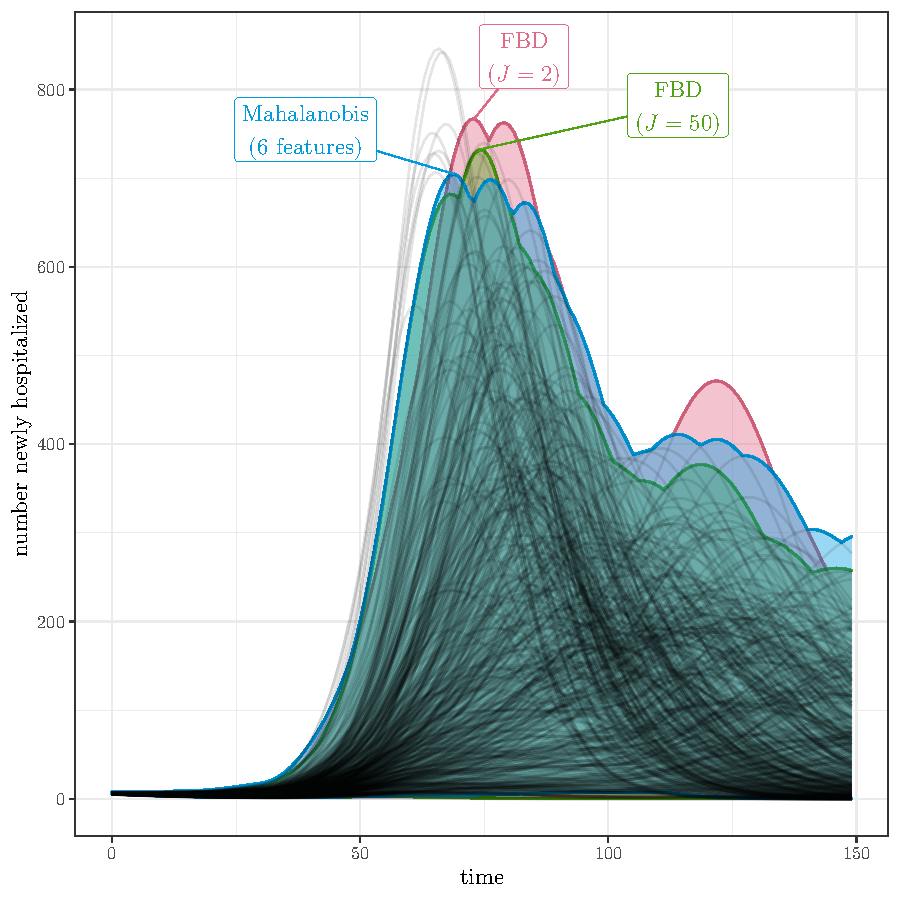
\includegraphics[width=\linewidth]{scripts/cent_plot.pdf}
  \caption{Comparison of 90\% central regions computed with
    different functional boxplot methods, using epidemic curve ensembles from \juul. FBD = functional band distance; $J$ = number of curves used for centrality calculation. Curve with $J=2$ computed via the \texttt{roahd} package \citep{roahd}: curve with $J=50$ used our own implementation of the functional band distance algorithm described by \juul, curve with Mahalanobis (5 features) used Mahalanobis distance on features of interest including the peak value of incidence, the time at which the peak occurs, the initial growth rate, epidemic duration, and final size of the epidemic.
  }
  \label{p.a}
\end{figure}
 
\section*{Discussion}

We compared definitions of central sets (and the resulting functional boxplots) based on band depths (based on pointwise 'betweenness' of curves) and on distances among sets of features derived from the curves, or between features of a curve and the centroid of sets of features for a given sample. For band-depth approaches, the only choices in defining a central set are (1) the size of the ensemble to use for ``betweenness'' --- FBDs using pairs, i.e. $J=2$, can be computed efficiently and seemed to give similar results to other choices for Juul et al's example --- and (2) questions of tie-breaking. For distance-based approaches, the primary choices are (1) what distance to use, (2) whether to measure distances among all sample points in a curve or between feature sets and (3) whether to base depth on \emph{average} pairwise distance among curves or distance to a centroid.

%% BMB: this paragraph is very confusing
%% In this work, we are computing the ``most central'' point in the set which we characterize as the point with minimum distance to all other points. The ``most central'' point is different from the concept of ``centroid''. In particular, in a space for a rank $r$, the (1) set of $r$ closest points to the centroid can be estimated (2) the set of $r$ points with the minimum average distance to all of the other points. We note that these two concepts can be different with respect to the choice of the norm, e.g., log Euclidean norm.

For some distance metrics (such as Euclidean distances), it is theoretically easy to define and computationally easy to compute a centroid; in contrast, measuring all pairwise distances among curves (so that depth can be defined as the average pairwise distance to other curves) is computationally expensive unless some efficient algorithm can be implemented. For our Mahalanobis calculations, we used the standard Euclidean centroid.

Mahalanobis distance computations also require a computation of the covariance matrix in order to scale elements of the distance appropriately; as described above, we used a covariance matrix based on the feature vectors for all observations in the data set. Such an approach could be misleading if the feature distribution is strongly bimodal or multimodal, in which case scaling factors derived from the overall data set may not be appropriate for scaling the components of distance between two trajectories whose features put them in the same mode of the distribution.

We briefly explored distance-based methods using all samples from the curve rather than feature vectors; we found that using a standard Euclidean distance ($\ell_2$ norm) tended to underestimate key features of epidemic ensemble such as the magnitude of epidemic peaks. Other well-known distances on spaces of functions, such as Fréchet distances and dynamic time warping, intentionally exclude differences based on phase (i.e., two curves that are identical up to a phase shift are considered to be coincident) --- this property seems inappropriate for evaluating ensembles of epidemic curves, but could be useful in other settings.

%% We also implemented a pairwise-distance approach, i.e., pairwise distances between the curves and quantiles of centrality, as an alternative method to a sampling-based functional boxplot. In particular, we compute all pairwise distances -- here we used $\ell_2$ norm which gives the area between the two curves -- between the curves, determine the median-like distance of a curve to all others as the minimum of sum of distances, and estimate the distribution of distances. We compared the 90\% most central region using the $\ell_2$ norm with the results from sampling-based method FBD and our proposed ranking method using Mahalanobis distance among features of interest (see appendix). We concluded that pairwise-distance approach using $\ell_2$ norm underestimated the key features of epidemic ensemble such as the magnitude of epidemic peaks.


\bibliography{./curveBP}

\section*{Appendix}

\begin{figure}[ht]\centering
  \includegraphics[width=\linewidth]{scripts/cent_plot2.pdf}
  \caption{Comparison of 90\% central regions computed with
    different functional boxplot and pairwise-distance methods, using epidemic curve ensembles from \juul. FBD = functional band distance; $J$ = number of curves used for centrality calculation. Curve with $J=2$ computed via the \texttt{roahd} package \citep{roahd}, curve with $J=50$ used our own implementation of the FBD algorithm described by \juul, curve with Mahalanobis (5 features) used Mahalanobis distance on features of interest including the peak prevalence, the time at which the peak occurs, the initial growth rate, epidemic duration, and total size of the epidemic.
  }
  \label{p.b}
\end{figure}
\end{document}
